% !TeX TXS-program:compile = txs:///pdflatex/[--shell-escape]
% Le truc au-dessus pour avoir l'option shell-escape qui permet de faire du minted.
\documentclass[12pt]{article}

% Affichage ou non des reponses aux questions & exercices
\newif\ifDispRep
%\DispReptrue  % Show the text
\DispRepfalse % Hide the text

% Version du document
\newcommand{\versiondoc}{v0.3}

% Incorporation tous éléments de préambule communs à tous mes cours
% Sans chemin relatif parce que TexStudio lancé depuis un script qui prend en compte la variable d'environnement TEXINPUTS
\usepackage{CoursLFC}

% Eléments de l'en-tête et de la page de garde spécifiques à ce doc
\newcommand{\classe}{1\textsuperscript{ère} NSI}
\newcommand{\themecours}{Exercices d'Entraînement}
\newcommand{\datedoc}{février 2024}

% Page de garde mise en page
\title
	{\vspace{2cm}
		{\Large
		\textit
			{
				\classe\hspace{0.1cm}
				\textemdash\
				\hspace{0.1cm}
				\themecours
			}
			
		\vspace{1cm}
		\huge{Algorithmique}
		
		\large{(et un peu de traitement de données en table / dictionnaires)}}
		 
		\vspace{1cm}
	}
\author{\etablissement}
\date{
	\auteur,
	\datedoc,
	\footnotesize{\textit{\versiondoc}} 
	\vspace{3cm}
	}

% Header & Footer
\lfoot{\etabshort}
\cfoot{\thepage}
\rfoot{\classe, \anneescol}
\renewcommand{\footrulewidth}{0.2pt}
\lhead{}
\chead{}
\rhead{}
\renewcommand{\headrulewidth}{0pt}

\begin{document}
	
	\maketitle
	% pas de footer sur la première page
	\thispagestyle{empty}
	\vspace{\baselineskip}
	\begin{MaReponse}
		\centering
		\vspace{\baselineskip}
		\textbf{Version incluant les réponses aux exercices.}
		\vspace{\baselineskip}
	\end{MaReponse}
	
	%\tableofcontents
	
	\pagebreak
	
	
	% Début du contenu du document
	%\section{Variants \& Invariants de boucles}
	\begin{MonExo}[Docstring \& Tests]
		Soit la fonction de calcul de puissance suivante (dont on a étudié l'algorithme en cours):
		\MonPython{Exos_001_PuissanceNoDocStrg.py}
		
		\begin{alphenum}
			\item Rédiger la docstring d'une telle fonction;
			\item Déterminer un jeu de tests pour cette fonction -- en d'autres termes, compléter le tableau suivant qui liste les couples (x, n) qu'il conviendra d'utiliser pour convenablement tester cette fonction.
		\end{alphenum}
		
		\centering
		\begin{tabular}{|c|c|c|}
			\hline
			\textbf{x} & \textbf{n} & \textbf{Résultat attendu}\\
			\hline
			2 & 2 & 4\\
			\hline
			...... & ...... & ......\\
			\hline
		\end{tabular}
	\end{MonExo}
	
	\begin{MaReponse}
		\MonPython{Exos_002_PuissanceDocStrg.py}
		Il n'y a pour le jeu de tests pas "une" bonne réponse, mais ce qu'on va chercher à faire c'est effectuer au moins deux tests de valeurs "normales" dont un avec une grande valeur (en plus, donc, du (2,2) de l'énoncé), ainsi que des tests avec les valeurs aux limites -- en l'occurrence 0 et 1 -- associées à des valeurs choisies au hasard. On pourra donc proposer quelque chose comme:
		
		\centering
		\begin{tabular}{|c|c|m{4cm}|}
			\hline
			\textbf{x} & \textbf{n} & \textbf{Résultat attendu}\\
			\hline
			2 & 2 & 4\\
			\hline
			27 & 7 & 10.460.353.203\\
			\hline
			21 & 0 & 1 (tout nombre élevé à la puissance 0 vaut 1)\\
			\hline
			35 & 1 & 35 \\
			\hline
			1 & 12 & 1 \\
			\hline
			0 & 99 & 0\\
			\hline
			0 & 0 & 1 (tout nombre élevé à la puissance 0 vaut 1 -- même 0)\\
			\hline
		\end{tabular}
	\end{MaReponse}


	\begin{MonExo}[Variant \& invariant de boucle]
		Soit la fonction suivante:
		\MonPython{Exos_003_SommeEltsListe.py}
		\begin{alphenum}
			\item Donner un variant de boucle pour cette fonction et montrer qu'elle se termine systématiquement;
			\begin{MonAmp}{Rappel}
				On rappelle qu'un variant de boucle est une quantité entière positive qui décroît strictement à mesure qu'on passe dans la boucle, ce qui permet de justifier que la boucle, tôt ou tard, se terminera.
			\end{MonAmp}
			\item Donner un invariant de boucle pour cette fonction et montrer qu'elle est correcte.
			\begin{MonAmp}{Rappel}
				On rappelle qu'un invariant de boucle est une quantité ou une propriété qui est vraie avant et après chaque itération de la boucle -- et en particulier \textit{avant} que l'on rentre dans la boucle, et \textit{après} sa dernière itération. Il permet de justifier que le résultat voulu sera atteint. On procède pour cette technique en quatre étapes:
				\begin{enumerate}
					\item On choisit l'invariant:
					\begin{itemize}
						\item Comprendre clairement le but de la boucle -- qu'est-elle censée accomplir? Quel est le résultat attendu?
						\item Partir "de la fin", c'est-à-dire du résultat attendu et identifier quelle quantité est "construite" au fur et à mesure des itérations de la boucle pour constituer ce résultat.
						\item Ceci devrait vous mettre sur la voie de votre invariant -- une propriété (somme d'éléments déjà traités, ordre d'éléments dans une liste...) qui ne change pas malgré les itérations de la boucle.
					\end{itemize}
					\item On montre que l’invariant est vérifié avant la boucle (initialisation);
					\item On montre que si l'invariant est vérifié \textit{avant }un passage dans la boucle, alors il est préservé \textit{après }le passage dans la boucle;
					\item On peut conclure sur la valeur finale à la sortie de la boucle.
				\end{enumerate}
			\end{MonAmp}
		\end{alphenum}
	\end{MonExo}
	
	\begin{MaReponse}
		\begin{alphenum}
			\item Variant de boucle -- on est dans le cas ultra-classique du parcours d'une liste par indice, le variant est donc la quantité $len(liste) - i - 1$: il est en effet positif au départ (au pire nul si la liste est vide), et il décroît strictement à chaque itération de la boucle puisque $len(liste)$ reste constant et que $i$ est incrémenté de 1 à chaque fois. Il va donc atteindre 0, ce qui terminera la boucle.
			\item Décomposons la démarche:
			\begin{enumerate}
				\item Choix de l'invariant: le but de la boucle est le calcul de la somme des éléments de la liste, et c'est la variable \texttt{res} qui est construite pour atteindre ce résultat: à chaque étape elle contient la somme des éléments d'indice de 0 à \texttt{i} de la liste. On peut donc dire que l'invariant de boucle est: "la variable \texttt{res} contient la somme des éléments d'indice de 0 à \texttt{i} de la liste";
				\item Avant la première itération de la boucle, \texttt{i} vaut 0 et \texttt{res} aussi -- donc on peut dire que l'invariant est vérifié;
				\item Si res contient les i premiers éléments de la liste et que l'on passe dans la boucle une fois supplémentaire, \texttt{i} et \texttt{res} deviennent respectivement: $i' = i + 1$ et $res' = res + liste[i'] = res + liste[i+1]$ -- et donc l'invariant est bien vérifié à la fin de l'itération de la boucle.
				\item A la fin de la boucle i vaut $(n-1)$ donc l'invariant s'exprime "la variable \texttt{res} contient la somme des éléments d'indice de 0 à \texttt{(n-1)} de la liste" -- soit tous les éléments de la liste, et donc la fonction est correcte.
			\end{enumerate}
		\end{alphenum}
	\end{MaReponse}

	\begin{MonExo}[Variant \& invariant de boucle --- suite...]
		Soit la fonction suivante:
		\MonPython{Exos_004_RechercheDiviseur.py}
		\begin{alphenum}
			\item Donner un variant de boucle pour cette fonction et montrer qu'elle se termine systématiquement;
			\item Donner un invariant de boucle pour cette fonction et montrer qu'elle est correcte.
			\begin{MonAmp}{Indice}
				On rappelle qu'un invariant de boucle n'est pas nécessairement une formule mathématique -- il peut aussi être une propriété que l'on pourrait exprimer par une phrase du genre (où bien entendu il faut remplir les trous): "Quel que soit l'entier k tel que 2 $\leq$ k $\leq$ \uline{\ \ \ \ }, k n'est pas\uline{\ \ \ \ }".
			\end{MonAmp}
			\item (question bonus 1) Cette boucle "\texttt{while}" semble assez artificielle -- on dirait presque qu'elle n'est là que pour vous forcer à travailler sur la notion de variant de boucle... Quelle est la boucle "\texttt{for}" équivalente qu'on utiliserait plus logiquement dans un tel cas?
			\item (question bonus 2) Cette fonction n'est pas franchement optimale... Comment remplacer la condition "\texttt{while i < nb:}" pour lui faire faire nettement moins de tests tout en gardant le bon résultat?
		\end{alphenum}
	\end{MonExo}
	
	\begin{MaReponse}
		\begin{alphenum}
			\item Variant de boucle -- situation assez simple: la quantité $nb - i$ débute à la valeur $nb - 2$ qui est nécessairement positive puisqu'il est spécifié que nb est strictement supérieur à 1; cette quantité décroît strictement à chaque itération de la boucle puisque $nb$ reste constant et que $i$ est incrémenté de 1 à chaque fois. Il va donc atteindre 0, ce qui terminera la boucle.
			\item Décomposons la démarche:
			\begin{enumerate}
				\item Choix de l'invariant: le but de la boucle est de trouver le diviseur le plus petit diviseur possible de nb, donc à chaque étape de la boucle, aucun nombre plus petit que celui que l'on est en train de considérer n'est diviseur de nb. On peut donc exprimer l'invariant: "quel que soit l'entier k tel que 2 $\leq$ k $\leq$ (i-1), k n'est pas un diviseur de nb";
				\item Avant la première itération de la boucle, \texttt{i} vaut 2, donc il n'existe aucun entier k tel que 2 $\leq$ k $\leq$ (i-1) -- donc on peut dire que l'invariant est vérifié;
				\item Si l'invariant est vérifié pour une valeur de i, alors pour la valeur suivante $i' = i + 1$, deux cas sont possibles:
				\begin{itemize}
					\item Soit i est un diviseur de nb et la fonction le renvoie et donc se termine (donc la question de l'invariant ne se pose plus);
					\item Soit i n'est pas un diviseur de nb -- et la boucle se poursuit et l'invariant est vérifié: "quel que soit l'entier k tel que 2 $\leq$ k $\leq$ (i'-1), k n'est pas un diviseur de nb" (puisque $i'-1 = i$).
				\end{itemize}
				\item A la fin de la boucle, dans l'hypothèse où on n'est pas sorti de la fonction, i vaut $nb$, donc l'invariant s'exprime "quel que soit l'entier k tel que 2 $\leq$ k $\leq$ (nb-1), k n'est pas un diviseur de nb" -- et donc nb est par définition un nombre premier.
			\end{enumerate}
			\item On fait varier i de 2 à nb-1 donc la boucle correspondante s'écrirait "\texttt{for i in range(2, nb)}".
			\item Il est évident que le plus grand diviseur d'un nombre (autre que lui-même) est sa moitié s'il est pair, ou son tiers s'il est impair mais un multiple de trois, etc. En tout état de cause, aucun nombre ne pourra avoir de diviseur strictement supérieur à sa moitié (ou la partie entière de sa moitié dans le cas d'un nombre impair). En écrivant la condition "\texttt{while i <= (nb // 2)}" on économiserait presque la moitié des opérations effectuées par la boucle tout en maintenant le résultat correct...
		\end{alphenum}
	\end{MaReponse}
	
	\begin{MonExo}[Variant \& invariant de boucle --- encore un!]
		Soit la fonction suivante:
		\MonPython{Exos_005_RechercheMax.py}
		Donner un invariant de boucle pour cette fonction et montrer qu'elle est correcte.
	\end{MonExo}
	
	\begin{MaReponse}
		\begin{enumerate}
			\item Choix de l'invariant: le but de la boucle est de trouver le maximum de la liste, donc avant chaque étape de la boucle, la variable \texttt{res} contient le maximum des éléments d'indice de 0 à \texttt{i-1} de la liste;
			\item Avant la première itération de la boucle, \texttt{i} vaut 0, donc la liste d'éléments dont l'indice est compris entre 0 et (i-1) est vide -- donc on peut dire que l'invariant est vérifié;
			\item Si l'invariant est vérifié pour une valeur de i, alors pour la valeur suivante $i' = i + 1$, deux cas sont possibles:
			\begin{itemize}
				\item Soit lst[i] $\leq$ res et donc, par définition, l'invariant reste vérifié (le maximum n'a pas changé);
				\item Soit lst[i] > res, res prend alors la valeur lst[i] qui est le nouveau maximum des éléments d'indice compris entre 0 et (i'-1) (donc i), et donc l'invariant est vérifié aussi.
			\end{itemize}
			\item A la fin de la dernière itération de la boucle, i vaut len(lst), donc res contient le maximum des éléments d'indice de 0 à \texttt{len(lst)-1} de la liste -- donc de toute la liste, et donc la boucle est correcte.
		\end{enumerate}
	\end{MaReponse}
	
	\begin{MonExo}[Complexité -- inversion de liste]
		Soit la fonction suivante:
		\MonPython{Exos_010_InvertLst.py}
		\begin{alphenum}
			\item Montrer, en utilisant un invariant de boucle, qu'elle fait bien ce que sa docstring spécifie.
			\item Compter son nombre d'opérations élémentaires, et en déduire sa complexité (préciser sa dénomination et sa notation en "$\mathcal{O}$").
		\end{alphenum}
	\end{MonExo}
	
	\begin{MaReponse}
		\begin{alphenum}
			\item L'invariant de boucle est la propriété, pour une valeur de i et après la réalisation de la boucle: "res est une liste contenant les i+1 derniers éléments de lst, dans l'ordre inverse". Initialisation: i=0, res contient uniquement lst[len(lst) - 1], soit le dernier élément de lst, donc l'invariant est vérifié. Si c'est vérifié pour i, lorsqu'on passe à i' = i + 1, on ajoute à la fin de res l'élément de lst d'indice (len(lst) - i' - 1) qui est le (i' + 1)\textsuperscript{ème} en partant de la fin, et on a donc rallongé res de 1 (sa longueur est donc maintenant i'+1) -- l'invariant est donc bien vérifié à i'. La boucle se termine lorsque i =  après len(lst) itérations, quand i est égal à len(lst) - 1, et donc à ce moment l'invariant s'exprime "res est une liste contenant les (len(lst)) derniers éléments de lst, dans l'ordre inverse" -- donc tous les éléments, et donc la boucle est correcte.
			\item Si l'on compte strictement les opérations on a:
			\begin{itemize}
				\item Deux opérations en dehors de la boucle (\texttt{res = []} et \texttt{return res});
				\item Une opération à l'intérieur de chaque itération de la boucle (le append sur la lsite res);
				\item Deux opérations à chaque itération de la boucle -- l'incrémentation de i et sa comparaison avec len(lst).
			\end{itemize}
			Si on note n la longueur de lst, la boucle est réalisée n fois et donc le nombre d'opérations est: $3 \times n + 2$ -- et donc on en déduit que la complexité est en $\mathcal{O}(n)$, c'est-à-dire linéaire.
		\end{alphenum}
	\end{MaReponse}

		\begin{MonExo}[Complexité -- note pondérée]
		Soit la fonction suivante:
		\MonPython{Exos_011_NotePonderee.py}
		Déterminer sa complexité.
	\end{MonExo}
	
	\begin{MaReponse}
		Aucun piège ici -- certes, on utilise len(lst\_notes) dans la fonction, mais pas dans le cadre d'une boucle. On n'exécute donc ici que deux opérations: le calcul de res et le return. On est donc dans une complexité constante, soit $\mathcal{O}(1)$.
	\end{MaReponse}
	
	\begin{MonExo}[Complexité -- somme de produits ou produit de sommes?]
		Soit les deux fonctions suivantes:
		\MonPython{Exos_007_ProdSomme.py}
		\MonPython{Exos_006_SommeProd.py}
		\begin{alphenum}
			\item Démontrer (simplement) que si j'applique ces deux fonctions aux mêmes paramètres n1 et n2 leur retour sera identique -- qu'en d'autres termes elles font le même calcul.
			\item Quelles sont les nombres d'opérations élémentaires qu'effectuent chacune de ces deux fonctions (exprimés en fonction de n1 et n2)? Laquelle des deux, du coup, vous semble la meilleure pour atteindre le résultat?
		\end{alphenum}
		
	\end{MonExo}
	
	\begin{MaReponse}
		\begin{alphenum}
			\item On voit de manière évidente que si l'on développe le produit de ProdSomme on tombera sur la somme de SommeProd:
			\begin{align*}
			\text{ProdSomme renvoie: } & [1 + 2 + (...) + (n_1 - 1)] \times [1 + 2 + (...) + (n_2 - 1)] \\
			\text{SommeProd renvoie: } & 1 \times 1 + 1 \times 2 + (...) + (n_1 - 1) \times (n_2 - 1)
			\end{align*}
			\item
			\begin{itemize}
				\item ProdSomme effectue successivement deux boucles de longueurs respectives n1 et n2 -- donc le nombre d'opérations élémentaires qu'elle va effectuer est de l'ordre de $n1 + n2$\footnote{Notez qu'ici on parle bien d'ordre de grandeur et qu'on néglige les opérations unitaires (comme le \texttt{res = 0} ou \texttt{return res}) qui ne changeront rien à la performance de la fonction quand on commencera à utiliser de grandes valeurs de n1 et n2.\label{Neglig}}.
				\item SommeProd, lui, effectue deux boucles \textit{imbriquées}: la boucle \textit{intérieure} (\texttt{for j in range(n2)}) va effectuer n2 itérations tandis que la boucle \textit{extérieure} (\texttt{for i in range(n1)}) va en effectuer n1 -- donc le nombre d'opérations élémentaires qu'elle va effectuer est de l'ordre de $n1 \times n2$\footref{Neglig}.
			\end{itemize}
			Il est donc évident que, pour des valeurs importantes de n1 et n2, ProdSomme sera \textit{beaucoup moins complexe} (et donc beaucoup plus performante) que SommeProd -- et ce pour le même résultat. Si on choisit par exemple n1 = 1.000.000 (un million) et n2 = 2.000.000 alors ProdSomme effectuera environ $n1 + n2 = 3.000.000$ d'opérations, tandis que SommeProd en effectuera environ $n1 \times n2 = 2.000.000.000.000$ (deux mille milliards) -- soit plus de 650.000 fois plus!
		\end{alphenum}
	\end{MaReponse}

		\begin{MonExo}[Tri à bulles - bidouillons-le un peu...]
		On rappelle le code Python du tri à bulles dans sa version la plus basique:
		\MonPython{007_TriBulles.py}
		\begin{alphenum}
			\item A quoi sert l'indice "i" dans cette fonction?
			\item Que se passe-t-il si on remplace la ligne 7 par \texttt{for j in range(n-1, -1, -1)}? Cette syntaxe  -- qui n'est rien de plus qu'une utilisation de la syntaxe \texttt{range} habituelle mais dans le contexte d'une suite décroissante) permet de réaliser une boucle allant de n-2 (le premier paramètre) à 0 (arrêt juste avant d'atteindre le deuxième paramètre) par pas de -1 (le troisième paramètre). L'indice va donc décrire la suite (n-2), (n-3), ..., 1, 0 au lieu de 0, 1, ..., (n-3), (n-2).
			\item Que se passe-t-il si on remplace la ligne 8 par \texttt{if liste[j] < liste[j+1]:}?
			\item La boucle interne ne fait-elle pas des opérations inutiles? Comment la modifier pour la rendre plus efficace?
		\end{alphenum}
		
	\end{MonExo}
	
	\begin{MaReponse}
		\begin{alphenum}
			\item Uniquement à compter le nombre de fois que l'on fait tourner la boucle interne! La variable i, comme on peut le constater, n'est utilisée nulle part hormis dans le \texttt{for} de la boucle.
			\item Eh bien... Rien du tout sur le résultat: on continue à échanger les éléments si celui de droite (d'indice supérieur) est inférieur à celui de gauche, donc on met à terme la liste dans le même ordre que précédemment. En revanche, on s'y prend dans l'autre sens, ce qui modifie la démarche: au lieu de faire "remonter" le plus grand élément du début à la fin de la liste, on va faire ici "descendre" le plus petit de la fin au début. Concrètement, si on passe en entrée la liste qu'on a utilisée en cours (\texttt{[2, 5, 3, 1]} ) on passera par les étapes suivantes:
			\begin{enumerate}
				\item \texttt{[2, 5, 3, 1]}
				\item \texttt{[1, 2, 5, 3]}
				\item \texttt{[1, 2, 3, 5]}
			\end{enumerate}
			\item Là, en revanche, on inverse le sens de tri -- on fait une permutation si l'élément de droite (d'indice supérieur) est \textbf{supérieur} à celui de gauche: donc on obtiendra à la fin la liste triée par ordre décroissant au lieu de croissant.
			\item A la fin de la première itération de la boucle externe (donc quand la boucle interne a fini son travail une première fois), on a ramené le plus grand élément de la liste à la fin de celle-ci; à la fin de la deuxième itération, le deuxième plus grand est en avant-dernière position; (...); à la fin de la i\textsuperscript{ième} itération, le i\textsuperscript{ième} plus grand est en i\textsuperscript{ième} position en partant de la fin, et tous ceux qui le suivent sont positionnés en ordre croissant (\textit{si vous ne me croyez pas, démontrez-le en utilisant un invariant de boucle -- c'est exactement à cela qu'ils servent!!}). Donc quand on passe à la (i+1)\textsuperscript{ième} itération de la boucle, on a déjà les i éléments "de droite" (de plus grands indices) de la liste qui sont déjà triés et qu'il ne sert plus à rien, de trier de nouveau --  on peut donc modifier la boucle interne pour qu'elle ne regarde plus ces éléments, et donc soit plus optimale, en la faisant aller non plus de 0 à n-2 mais de 0 à n-i-2. Le résultat sera le suivant:
			\MonPython{Exos_012_TriBullesOptim.py}
		\end{alphenum}
	\end{MaReponse}
	


	\begin{MonExo}[Devinette de nombre]
		Le code utilisé pour l'implémentation de la fonction de recherche dichotomique est le suivant:
		\MonPython{011_RechDich.py}
		Appuyez-vous sur cette approche et développez le jeu évoqué en cours -- vous choisissez un nombre entre 0 et 100 et l'ordinateur doit le deviner en vous posant des questions.
		
		\vspace{\baselineskip}
		Exemple de séquence:
		\begin{verbatim}
			Pensez à un nombre entre 0 et 100...
			Si il est plus grand que 50, tapez 1; s'il est plus petit, tapez 2;
			s'il est égal à 50 tapez 3.
			2
			Si il est plus grand que 25, tapez 1; s'il est plus petit, tapez 2;
			s'il est égal à 25 tapez 3.
			3
			J'ai trouvé! Votre nombre est 25.
		\end{verbatim}
		
		\vspace{\baselineskip}
		Indices:
		\begin{itemize}
			\item Vous allez évidemment devoir utiliser la fonction "input()" pour recueillir les réponses de l'utilisateur;
			\item Vous allez construire de nombreuses fois le même message, avec des valeurs différentes. Voici un exemple qui pourra vous aider:
			\begin{figure}[H]
				\centering
				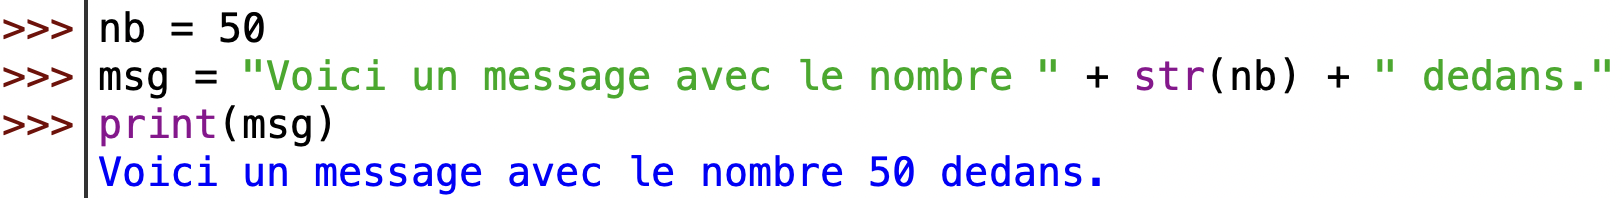
\includegraphics[width=0.9\textwidth]{048_Concat.png}
			\end{figure}
		\end{itemize}
		%\vspace{1.5\baselineskip}
		\vspace{\baselineskip}
		\textit{Version améliorée: l'ordinateur doit être capable de détecter si l'utilisateur triche (change de nombre en cours de route)...}
	\end{MonExo}
	\begin{MaReponse}
		Le code demandé ici est relativement simple:
		\MonPython{Exos_013_RechNb.py}
		
		Pour ce qui est de la version améliorée, il est impossible de détecter que l'utilisateur a menti tant qu'on n'a pas fini l'algorithme: en effet, à tout moment, tant que \texttt{debut <= fin}, on n'a pas couvert la totalité des nombres possibles et donc le nombre deviné par l'utilisateur peut en être un qu'on n'a pas encore couvert. En revanche, si l'on termine l'algorithme sans avoir trouvé (lorsque \texttt{debut > fin}), on est forcément dans un cas où l'utilisateur a triché (puisque, on l'a démontré en cours, l'algorithme est correct). On peut donc, après la boucle, ajouter un message pour dire à l'utilisateur qu'on l'a capté!
	\end{MaReponse}

	\begin{MonExo}[Recherche dichotomique]
		Donnez deux exemples d'exécution de recherche dichotomique où le nombre d'exécutions de la boucle est exactement 4 --- un sans solution (retour de $-1$), une avec une solution. Dans les deux cas il vous est demandé de donner la liste considérée et le nombre recherché.
	\end{MonExo}
	\begin{MaReponse}
		Le cas le plus simple est celui où l'on ne trouve pas la valeur cherchée: en effet, comme on l'a vu en cours, c'est le cas le pire du point de vue de la complexité, et dans ce cas elle est en $\mathcal{O}(log_2(n))$. Donc pour avoir 4 opérations, il faut une liste de longueur $2^4 = 16$. Donc, par exemple, la recherche de "20" dans la liste \texttt{[1, 2, 3, 4, 5, 6, 7, 8, 9, 10, 11, 12, 13, 14, 15, 16]} se fera en 4 itérations.
		
		Si l'on y réfléchit bien, le cas où l'on va trouver l'élément (si on ne demande pas plus de conditions comme c'est le cas ici) n'est pas beaucoup plus simple puisque l'algorithme de la recherche dichotomique est construit de telle sorte que les derniers éléments à être considérés sont les extrémités du tableau. On peut donc dire que la recherche de "1" (tout comme celle de "16") dans la liste \texttt{[1, 2, 3, 4, 5, 6, 7, 8, 9, 10, 11, 12, 13, 14, 15, 16]} se fera en 4 itérations.
	\end{MaReponse}
	
	\begin{MonExo}[Recherche dichotomique modifiée]
		\begin{alphenum}
			\item  Modifier l'algorithme de recherche dichotomique afin qu'il indique le nombre valeurs examinées dans un tableau donné pour localiser un élément dans un tableau trié ou indiquer qu'il n’est pas présent dans le tableau
			\item Quels tests peut-on imaginer pour cet algorithme ?
		\end{alphenum}
	\end{MonExo}
	\begin{MaReponse}
		\begin{alphenum}
			\item La modification de l'algorithme est simple -- il suffit d'ajouter un compteur et de l'afficher (très similaire à ce que l'on a fait avec la variable \texttt{cps} dans l'exercice 9 ci-dessus). Notez:
			\begin{itemize}
				\item Les lignes 4, 8, et 10 de l'algorithme ci-dessous où l'on implémente le compteur;
				\item La ligne 7 où l'on stocke T[Milieu] dans une variable, ce qui nous permet de l'utiliser plusieurs fois en ne la lisant qu'une seule fois.
			\end{itemize} 
			
			\begin{algorithmic}[1]
				\Require{$T$, $x$}
				\Ensure{$position$ de l'élément $x$ dans $T$, -1 si non trouvé}
				\Function{RechDichotomique}{$T$, $x$}
				\State $Debut$ $\leftarrow 1$
				\State $Fin$ $\leftarrow longueur(T)$
				\State $ValLues$ $\leftarrow 0$
				\While{$Debut \leq Fin$}
				\State $Milieu$ $\leftarrow (Debut + Fin) // 2$
				\State $ValCur$ $\leftarrow T[Milieu]$
				\State $ValLues$ $\leftarrow ValLues + 1$
				\If{$x = ValCur$}
				\Comment{On a trouvé l'élément recherché}
				\State Afficher "On a lu: " $ValLues$ " valeurs dans le tableau"
				\State\Return{$Milieu$}
				\ElsIf{$x > ValCur$}
				\State $Debut$ $\leftarrow Milieu + 1$
				\Comment{L'élément n'est pas "à gauche"}
				\Else
				\State $Fin$ $\leftarrow Milieu - 1$
				\Comment{L'élément n'est pas "à droite"}
				\EndIf
				\EndWhile
				\State\Return{$-1$}
				\Comment{On ne l'a pas trouvé}
				\EndFunction
			\end{algorithmic}
			\item Pour les tests à effectuer il importe d'essayer de couvrir le plus de cas possibles. On peut par exemple imaginer un jeu de tests contenant:
			\begin{itemize}
				\item Une recherche de 2 dans \texttt{L = [1, 2, 3, 4, 5, 6]} (valeur trouvée, qui n'est pas à une extrémité);
				\item Une recherche de 5 dans \texttt{L} (valeur non trouvée);
				\item Une recherche de 1 puis 4 dans \texttt{L} (valeur trouvée, qui est à une extrémité);
				\item Recherche de 1 dans \texttt{LVide = []} (liste vide).
			\end{itemize}
		\end{alphenum}
	\end{MaReponse}
	
	\begin{MonExo}[Jeu des 7 différences (enfin 2 en l'occurrence...)]
		Soit le code suivant:
		\MonPython{Exos_014_RechDichFausse.py}
		Voyez-vous les deux différences entre ce code et celui qu'on a développé en cours? Quel problème est-ce que cela pose? Que se passerait-il si je lançais la commande \texttt{RechDich([1, 2, 3, 4, 5], 5)}?
	\end{MonExo}
	\begin{MaReponse}
		Les différences se situent aux lignes 12 et 14 du code où l'on a \texttt{debut = milieu} et \texttt{fin = milieu} au lieu de \texttt{debut = milieu + 1} et \texttt{fin = milieu - 1} respectivement. Ceci pourrait entrainer une boucle infinie dans certains cas comme on va le voir sur l'exemple proposé dans l'énoncé (comme on travaille ici sur du code Python et non du pseudo-code j'utilise les indices de 0 à n):
		
		\begin{tabular}{|c|c|c|c|}
			\hline
			\textbf{Debut} & \textbf{Fin} & \textbf{Milieu} & \textbf{\texttt{liste[Milieu]}}\\
			\hline
			0 & 4 & 2 & 3\\
			\hline 
			2 & 4 & 3 & 4 \\
			\hline 
			3 & 4 & 3 & 4 \\
			\hline
			3 & 4 & 3 & 4 \\
			\hline
			\multicolumn{4}{c}{\textbf{etc.............}} 
		\end{tabular}
		
		Vous remarquerez que c'est le seul cas où le problème se posera --- une recherche de n'importe quelle autre valeur fonctionnera sans problème.
	\end{MaReponse}
	
	\begin{MonExo}[Une fonction tordue]
		On considère le code de fonction suivant:
		\MonPython{Exos_015_NbrDup.py}
		\begin{alphenum}
			\item A la main, déterminez le résultat de l'appel à cette fonction pour les cas suivants:
			\begin{enumerate}
				\item \texttt{t = [1, 2, 3]}
				\item \texttt{t = [1, 1, 1]}
				\item \texttt{t = [1, 1, 3]}
				\item \texttt{t = [1, 2, 2]}
			\end{enumerate}
			\item Comment, du coup, formuleriez-vous la \texttt{docstring} de cette fonction pour expliquer ce qu'elle fait?
			\item En termes de complexité (donc du nombre d'opérations effectuées par la fonction), lequel des 4 cas suivants est le pire?
			\item On se place dans un cas "au pire": combien de fois, en fonction de $n$ la taille du tableau \texttt{t}, l'instruction \texttt{n\_dup[i] += 1} est-elle effectuée lorsque:
			\begin{enumerate}
				\item $i$ vaut $0$?
				\item $i$ vaut $1$?
				\item $i$ vaut $n - 1$?
			\end{enumerate}
			\item En déduire, en justifiant bien, la complexité en fonction de $n$ de la fonction \texttt{NbrDup}.
		\end{alphenum}
	\end{MonExo}
	\begin{MaReponse}
		\begin{alphenum}
			\item Reprenons l'approche que nous avons déjà utilisée plus haut, à savoir un tableau qui nous permet de suivre les valeurs successives de différentes variables:
			\begin{enumerate}
				\item Pour \texttt{t = [1, 2, 3]}:
				
				\begin{tabular}{|c|c|c|c|c|c|}
					\hline
					\textbf{Ligne Code} & \texttt{n\_dup} & \texttt{i} & \texttt{j} & \texttt{t[i]} & \texttt{t[j]} \\
					\hline
					6 & \texttt{[0,0,0]} & - & - & - & -\\
					\hline 
					9 & \texttt{[0,0,0]} & 0 & 1 & 1 & 2\\
					\hline 
					9 & \texttt{[0,0,0]} & 0 & 2 & 1 & 3\\
					\hline 
					9 & \texttt{[0,0,0]} & 1 & 2 & 2 & 3\\
					\hline 
				\end{tabular}
				
				Et le traitement renvoie donc \texttt{[0,0,0]}
				
				\item Pour \texttt{t = [1, 1, 1]}:
				
				\begin{tabular}{|c|c|c|c|c|c|}
					\hline
					\textbf{Ligne Code} & \texttt{n\_dup} & \texttt{i} & \texttt{j} & \texttt{t[i]} & \texttt{t[j]} \\
					\hline
					6 & \texttt{[0,0,0]} & - & - & - & -\\
					\hline 
					9 & \texttt{[0,0,0]} & 0 & 1 & 1 & 1\\
					\hline 
					10 & \texttt{[1,0,0]} & 0 & 1 & 1 & 1\\
					\hline 
					9 & \texttt{[1,0,0]} & 0 & 2 & 1 & 1\\
					\hline 
					10 & \texttt{[2,0,0]} & 0 & 1 & 1 & 1\\
					\hline 
					9 & \texttt{[2,0,0]} & 1 & 2 & 1 & 1\\
					\hline 
					10 & \texttt{[2,1,0]} & 0 & 1 & 1 & 1\\
					\hline 
				\end{tabular}
				
				Et le traitement renvoie donc \texttt{[2,1,0]}
				
				\item Pour \texttt{t = [1, 1, 3]}:
				
				\begin{tabular}{|c|c|c|c|c|c|}
					\hline
					\textbf{Ligne Code} & \texttt{n\_dup} & \texttt{i} & \texttt{j} & \texttt{t[i]} & \texttt{t[j]} \\
					\hline
					6 & \texttt{[0,0,0]} & - & - & - & -\\
					\hline 
					9 & \texttt{[0,0,0]} & 0 & 1 & 1 & 1\\
					\hline 
					10 & \texttt{[1,0,0]} & 0 & 1 & 1 & 1\\
					\hline 
					9 & \texttt{[1,0,0]} & 0 & 2 & 1 & 3\\
					\hline 
					9 & \texttt{[1,0,0]} & 1 & 2 & 1 & 3\\
					\hline 
				\end{tabular}
				
				Et le traitement renvoie donc \texttt{[1,0,0]}
				
				\item Pour \texttt{t = [1, 2, 2]}:
				
				\begin{tabular}{|c|c|c|c|c|c|}
					\hline
					\textbf{Ligne Code} & \texttt{n\_dup} & \texttt{i} & \texttt{j} & \texttt{t[i]} & \texttt{t[j]} \\
					\hline
					6 & \texttt{[0,0,0]} & - & - & - & -\\
					\hline 
					9 & \texttt{[0,0,0]} & 0 & 1 & 1 &2\\
					\hline 
					9 & \texttt{[0,0,0]} & 0 & 2 & 1 & 2\\
					\hline 
					9 & \texttt{[0,0,0]} & 1 & 2 & 2 & 2\\
					\hline 
					10 & \texttt{[0,1,0]} & 1 & 2 & 2 & 2\\
					\hline 
				\end{tabular}
				
				Et le traitement renvoie donc \texttt{[0,1,0]}
			\end{enumerate}
			
			\item On pourrait écrire (mais je vous accorde que c'est bien tordu...):
			\begin{verbatim}
				''' Fonction qui prend en entrée un tableau t et qui renvoie 
				un tableau n_dup de même taille que t qui contient, à chaque 
				indice, le nombre de fois que t[i] est présent dans la suite 
				du tableau (donc dans les indices [i+1, n-1]).'''
			\end{verbatim}
			
			\item La réponse est à la fois logique et facile à constater en regardant les tableaux ci-dessus. La seule instruction qui n'est pas effectuée à chaque fois est \texttt{n\_dup[i] += 1} puisqu'elle dépend de la condition \texttt{if t[i] == t[j]}; le cas le pire est donc celui où cette condition est vérifiée un maximum de fois --- donc dans le cas (b) ci-dessus, celui où toutes les valeurs du tableau sont identiques. Ceci se vérifie aisément en constatant le nombre de lignes des tableaux qu'on a utilisés ci-dessus, qui est maximal dans le cas (b).
			
			\item On se place donc ici dans le cas d'un tableau de longueur $n$ contenant $n$ fois la même valeur (voir ci-dessus: cas le pire, celui où la condition \texttt{if t[i] == t[j]} est vérifiée à chaque itération de la boucle). 
			
			\begin{enumerate}
				\item Si $i = 0$ alors $j$ ira de 1 à $(n-1)$ et donc l'instruction sera exécutée $(n-1)$ fois.
				\item Si $i = 1$ alors $j$ ira de 2 à $(n-1)$ et donc l'instruction sera exécutée $(n-2)$ fois.
				\item Si $i = (n - 1)$ alors $j$ ira de $n$ à $(n-1)$ et donc l'instruction ne sera pas exécutée du tout (exécutée 0 fois).
			\end{enumerate}
			
			\item On peut généraliser ce que l'on vient de calculer en disant que lorsqu'on a $i = k$, l'instruction \texttt{n\_dup[i] += 1} est exécutée exactement $(n - 1 - k)$ fois. Donc si l'on regarde le traitement dans son ensemble le nombre d'exécutions de l'instruction sera:
			
			\begin{align*}
				(n - 1) + (n - 2) + \text{(...)} + 2 + 1 + 0 &= \frac{n\times (n-1)}{2} \\
				&= \frac{1}{2} \times n^2 - n \times \frac{1}{2}
			\end{align*}
			
			La complexité de la fonction dépend donc du carré de $n$, elle est donc quadratique et se note "$\mathcal{O}(n^2)$".
		\end{alphenum}
	\end{MaReponse}
	
	\begin{MonExo}[Un peu de travail sur les dictionnaires]
		On considère le code de fonction suivant:
		\MonPython{Exos_016_Occ.py}
		\begin{alphenum}
			\item \textbf{\textit{Encore}} une fonction où on a oublié de mettre la \texttt{docstring}!! Que proposez-vous?
			\item Ecrire une fonction \texttt{compare\_tableaux(t, u)} qui prend deux tableaux \texttt{t} et \texttt{u} en entrée et détermine si ils contiennent les mêmes éléments, mais sans les trier.
		\end{alphenum}
	\end{MonExo}
	\begin{MaReponse}
		\begin{alphenum}
			\item Cette fonction prend un tableau en entrée et renvoie en sortie un dictionnaire avec tous les éléments distincts présents dans le tableau ainsi que le nombre d'occurrences de chacun de ces éléments.
			
			\item Il est évident que la fonction précédente ne nous a pas été fournie par hasard -- on va s'appuyer dessus pour rédiger la fonction \texttt{compare\_tableaux}:
			\MonPython{Exos_017_CompTab.py}
		\end{alphenum}
	\end{MaReponse}
	
	\begin{MonExo}[Ah tiens au fait...]
		Est-ce que la fonction \texttt{Occ} qu'on a vue à l'exercice précédent fonctionnerait si on lui passait en entrée une chaine de caractères au lieu d'une liste? Que renverrait l'appel \texttt{Occ("abracadabra")}?
		
		Qu'en serait-il de \texttt{compare\_tableaux} si on lui passait deux chaines de caractères en entrée?
	\end{MonExo}
	\begin{MaReponse}
		Dans \texttt{Occ} on ne "touche" à la variable passée en argument qu'une seule fois, dans la boucle principale "\texttt{for x in t}" -- et on a vu en cours qu'on peut tout à fait parcourir une chaîne de caractères de cette manière. Donc l'appel \texttt{Occ("abracadabra")} fonctionnerait bien et renverrait \texttt{\{'a': 5, 'b': 2, 'r': 2, 'c': 1, 'd': 1\}}.
		
		Dans \texttt{compare\_tableaux}, on "touche" à nos variables en entrée deux fois:
		\begin{itemize}
			\item Via la fonction \texttt{len} -- dont on a vu en cours qu'elle fonctionne très bien avec les chaines de caractère;
			\item Via la fonction \texttt{Occ} -- qu'on vient de regarder.
		\end{itemize}
		Donc en dépit de son nom \texttt{compare\_tableaux} fonctionnerait très bien avec des chaines de caractères.
	\end{MaReponse}
	
	\begin{MonExo}[Tris décroissants]
		\begin{alphenum}
			\item Ré-écrire l'algorithme du tri par sélection tel qu'on l'a vu en cours pour qu'il produise un tri par ordre décroissant;
			\item Même chose avec l'algorithme de tri par insertion.
		\end{alphenum}
	\end{MonExo}
	\begin{MaReponse}
		\begin{alphenum}
			\item Il suffit de substituer la notion de maximum à la notion de minimum pour inverser l'ordre du tri dans le tri par sélection:
			\begin{algorithmic}[1]
				\Require{$tab$, une liste}
				\Ensure{$tab$, triée}
				\Function{TriSelection}{tab}
				\State n $\leftarrow$ longueur(tab)
				\For{$p$ allant de 1 à (n-1)}
				\State pmax $\leftarrow$ p
				\For{$j$ allant de (p+1) à n}
				\If{$tab[j] > tab[pmax]$}
				\Comment{On a trouvé un nouveau max}
				\State $pmax$ $\leftarrow j$
				\EndIf
				\EndFor
				\State Échanger tab[pmax] et tab[p]
				\EndFor
				\State\Return{$tab$}
				\EndFunction
			\end{algorithmic}
			
			\item Dans le tri par insertion, c'est encore plus simple: lorsqu'on remonte la partie déjà triée du tableau, on se contente de chercher l'indice où \texttt{temp} dépasse \texttt{tab[p-1]} et on insère temp à cet endroit (la seule ligne impactée est la ligne 6 où l'on a remplacé un ">" par un "<"):
			\begin{algorithmic}[1]
				\Require{$tab$, une liste}
				\Ensure{$tab$, triée}
				\Function{TriInsertion}{tab}
				\State n $\leftarrow$ longueur(tab)
				\For{$i$ allant de 2 à n}
				\State temp $\leftarrow$ tab[i]
				\State p $\leftarrow$ i
				\While{$p > 1$ et tab[p-1] < temp}
				
				\Comment{On remonte le tableau jusqu'à trouver la place de tab[i]}
				\State tab[p] $\leftarrow$ tab[p-1]
				\State p $\leftarrow$ p-1
				\EndWhile
				\State tab[p] $\leftarrow$ temp
				\Comment{On a trouvé la place de tab[i]}
				\EndFor
				\State\Return{$tab$}
				\EndFunction
			\end{algorithmic}
		\end{alphenum}
	\end{MaReponse}
	
	\begin{MonExo}[Un festival glouton]
		Vous venez d'arriver au Festival d'Avignon et découvrez qu'il se déroule sur 5 scènes différentes, avec une programmation extrêmement complexe:
		\begin{figure}[H]
			\centering
			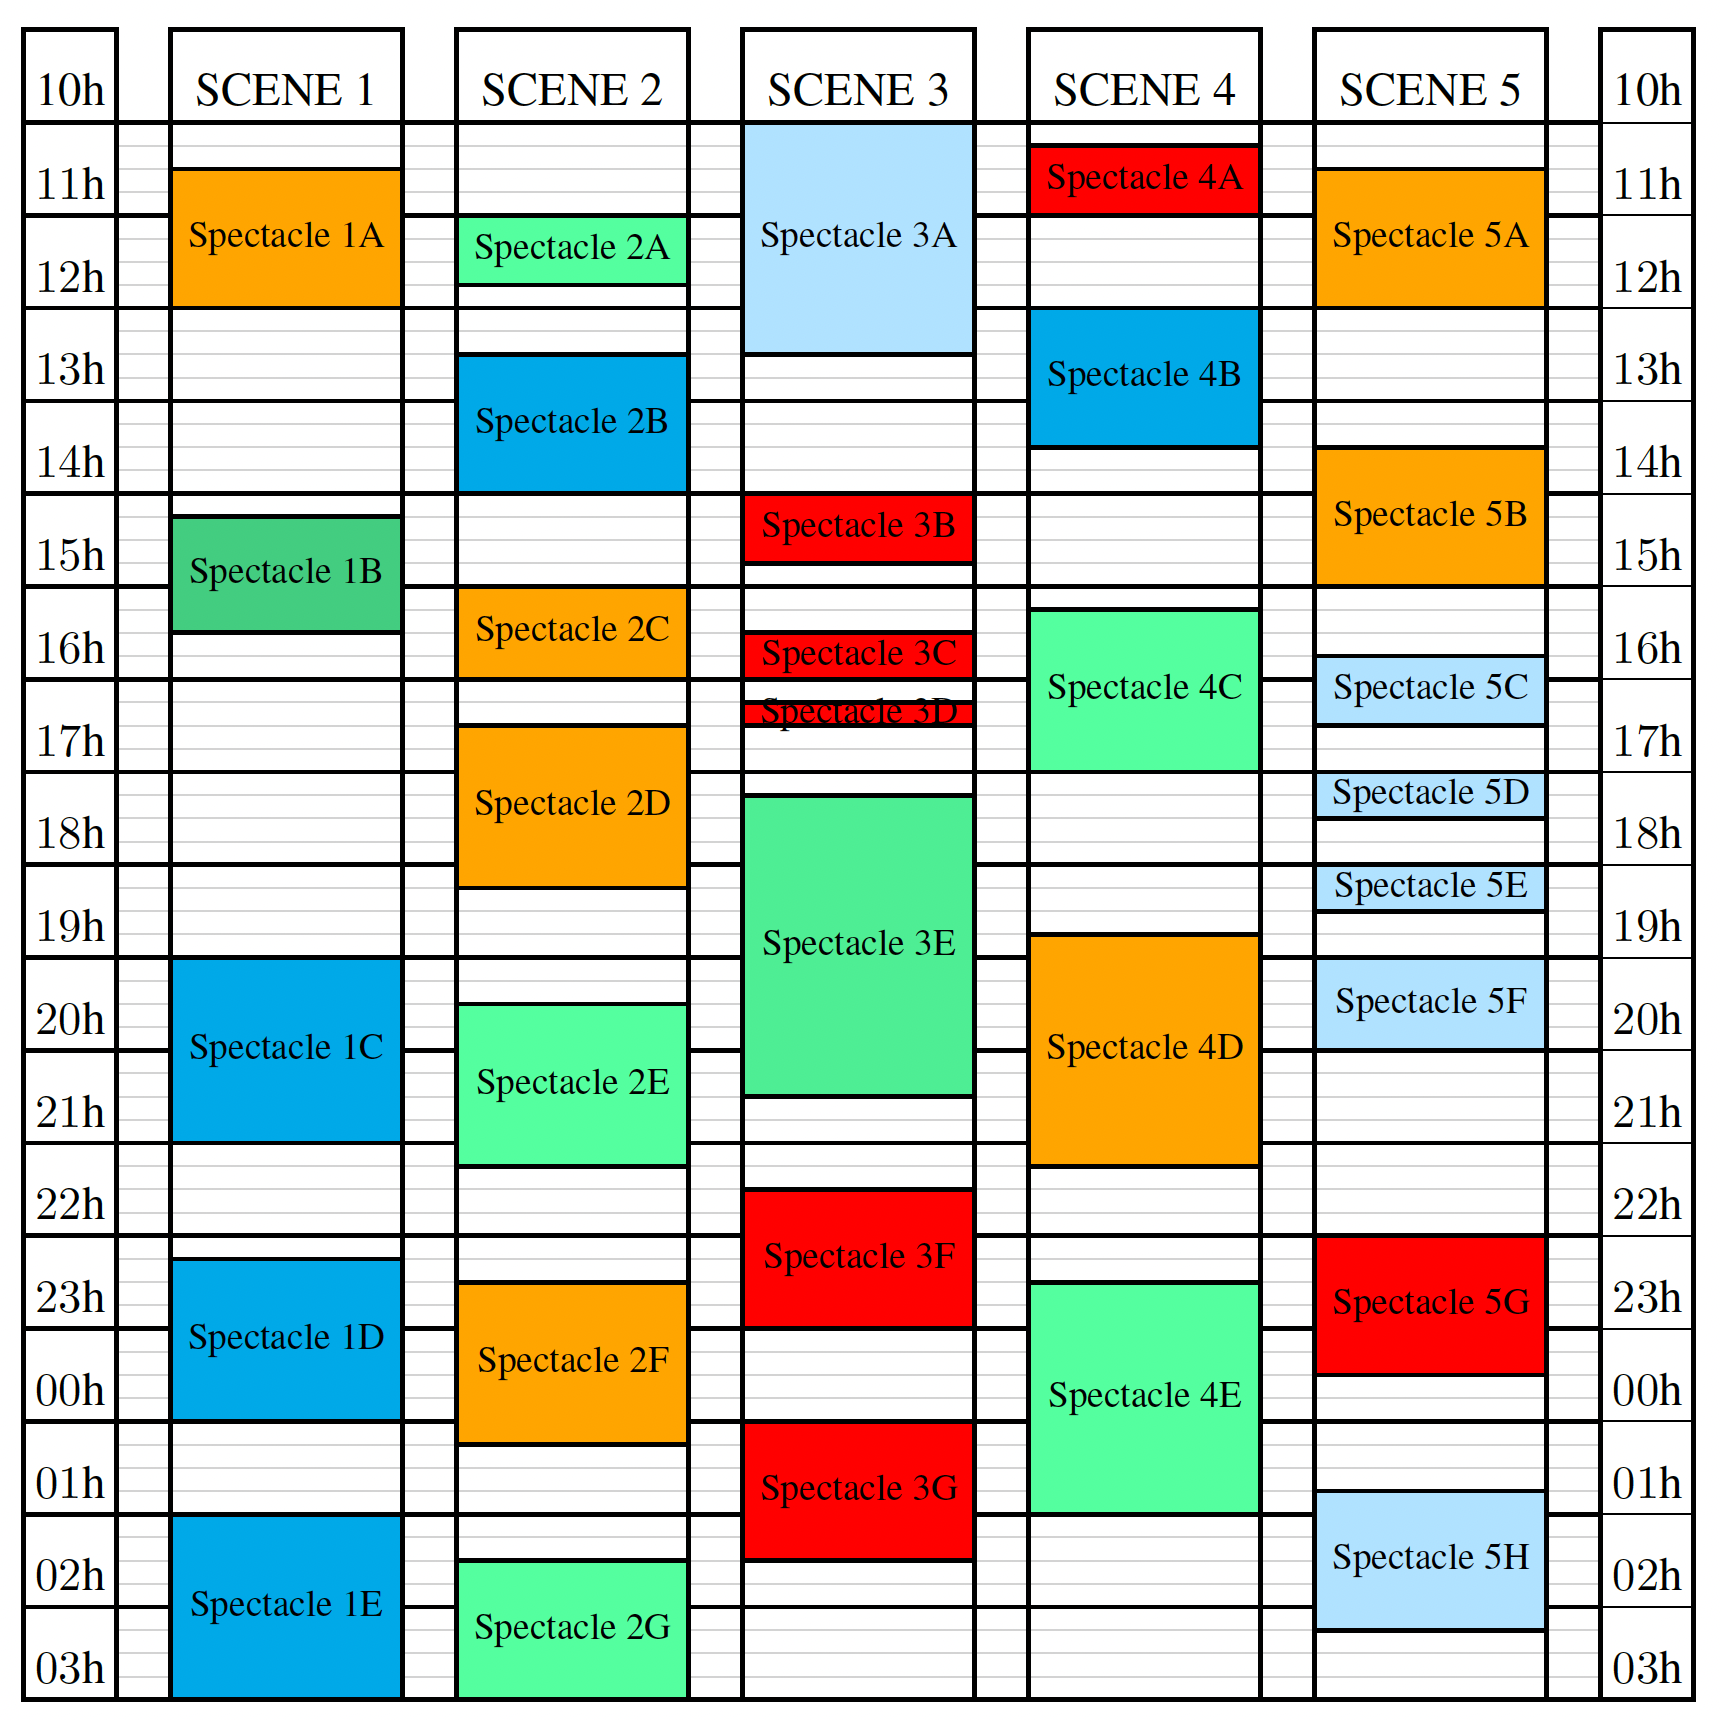
\includegraphics[width=\textwidth]{050_Avignon.png}
		\end{figure}
		Brillant élève de NSI que vous êtes, vous vous décidez à choisir les spectacles auxquels vous allez assister en appliquant une méthode gloutonne. Les règles à respecter sont:
		\begin{itemize}
			\item Vous voulez voir le nombre maximal possible de spectacles dans la journée;
			\item Lorsque vous commencez un spectacle vous voulez le voir en entier (du début à la fin);
			\item On suppose que le temps de trajet entre les scènes est nul.
		\end{itemize}
		
		On va considérer deux algorithmes gloutons séparés: appliquez le déroulé de chacun d'entre eux et concluez sur celui qui fonctionne le mieux.
		\begin{alphenum}
			\item Algorithme A: moins on attend entre deux spectacles plus on en verra, donc à chaque étape on choisit le prochain spectacle qui débute le plus tôt.
			\item Algorithme B: plus chaque spectacle que l'on voit finit tôt plus on aura de temps pour voir d'autres spectacles, donc à chaque étape on choisit le prochain spectacle qui finit en premier.
		\end{alphenum}
	\end{MonExo}
	\begin{MaReponse}
		\begin{alphenum}
			\item Algorithme A:
			\begin{description}
				\item[Etape 1] 3A
				\item[Etape 2] 2B
				\item[Etape 3] 3B
				\item[Etape 4] 2C
				\item[Etape 5] 3D
				\item[Etape 6] 2D
				\item[Etape 7] 4D
				\item[Etape 8] 3F
				\item[Etape 9] 3G
				\item[Etape 10] 2G
			\end{description}
			\item Algorithme B:
			\begin{description}
				\item[Etape 1] 4A
				\item[Etape 2] 2A
				\item[Etape 3] 4B
				\item[Etape 4] 3B
				\item[Etape 5] 2C ou 3C
				\item[Etape 6] 3D
				\item[Etape 7] 5D
				\item[Etape 8] 5E
				\item[Etape 9] 5F
				\item[Etape 10] 3F
				\item[Etape 11] 3G
				\item[Etape 12] 2G
			\end{description}
		\end{alphenum}
		Et on conclut donc que l'approche B est mieux optimisée que l'approche 1A.
	\end{MaReponse}
	
	\begin{MonExo}[Encore un peu d'algorithmes gloutons...]
		On considère la figure ci-dessous:
		\begin{figure}[H]
			\centering
			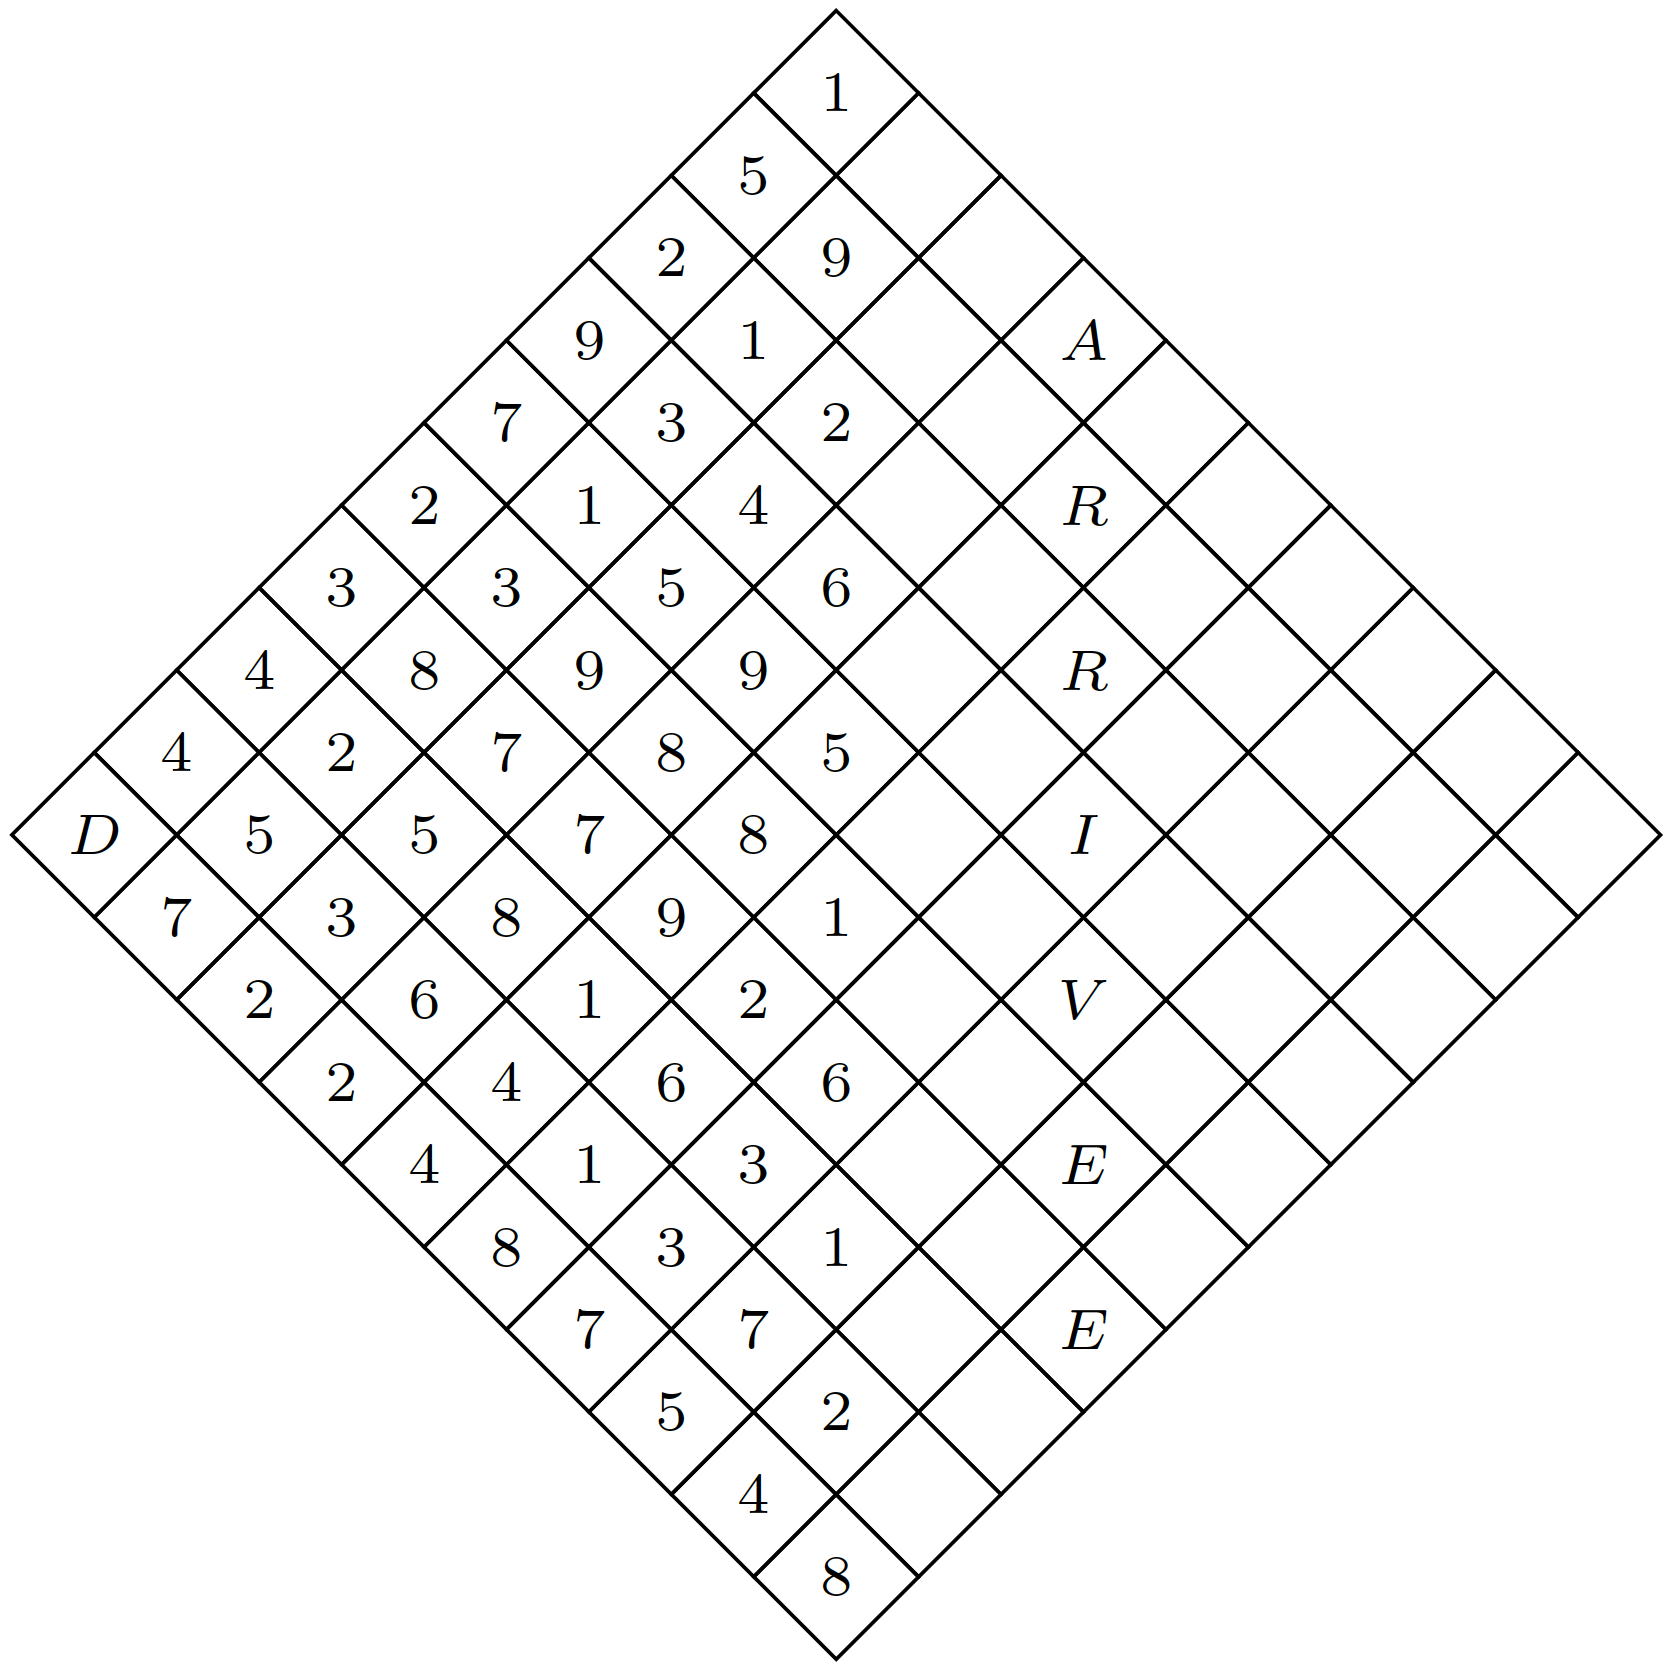
\includegraphics[width=0.7\textwidth]{051_TabGlouton.png}
		\end{figure}
		Le jeu sur cette grille consiste à partir n part de la case "\textbf{D}" à gauche et de se rendre sur une des cases vides à droite en se déplaçant de case en case. Lorsqu'on est sur une case on peut se déplacer sur une des deux cases voisines situées sur la droite, mais pas sur la case reliée uniquement par un sommet (donc de la case D on peut aller en 4 ou en 7 mais pas en 5).
		
		On note S la somme de toutes les cases traversées. Par exemple on peut effectuer la trajectoire suivante: \texttt{D - 7 - 5 - 3 - 5 - 7 - 9 - 8 - 9 - 6} qui donne $S = 59$.
		
		Le but du jeu est d'effectuer la trajectoire qui rend la somme S la plus petite possible.
		
		\begin{alphenum}
			\item Décrivez une approche gloutonne à la résolution de ce problème. Combien de calculs sont nécessaires pour choisir la trajectoire?
			\item En appliquant cette approche, quelle trajectoire et quelle somme S obtenez-vous?
			\item Sur cette grille, en cherchant bien, la trajectoire optimale donne une somme $S = 23$. Votre algorithme glouton a-t-il trouvé cette trajectoire optimale? Si la réponse est non, est-ce que la trajectoire trouvée vous semble proche de la trajectoire optimale?
			\item Comment pourrait-on modifier l'algorithme pour l'améliorer? Combien de calculs sont nécessaires pour choisir la trajectoire avec cette amélioration?
			\item Pour être sûr d'obtenir la solution optimale cependant, il n'y a d'autre choix que d'adopter une approche "force brute" -- regarder toutes les trajectoires possibles et choisir celle au score le plus faible. Démontrer qu'on va devoir calculer 512 trajectoires.
calculs.
		\end{alphenum}
	\end{MonExo}
	\begin{MaReponse}
		\begin{alphenum}
			\item A chaque étape on a le choix entre deux cases: on va systématiquement choisir celle de valeur inférieure et, en cas d'égalité, on va en choisir une au hasard. Toutes les trajectoires ont 9 étapes donc on va effectuer 9 comparaisons avant d'obtenir notre trajectoire.
			\item \texttt{D - 4 - 4 - 2 - 5 - 7 - 7 - 8 - 8 - 5}, pour $S = 50$.
			\item Il est évident que notre algorithme n'a pas trouvé la meilleure trajectoire, et d'assez loin.
			\item On pourrait, à chaque coup, regarder les deux cases suivantes --- donc 4 combinaisons à comparer --- et choisir la case qui fournit la combinaison la plus faible. Par exemple, en partant de D, les premières étapes seraient:
			\begin{itemize}
				\item Quatre premières combinaisons possibles: 4-4, 4-5, 7-5, 7-2. La combinaison la plus faible est la première (8), donc on choisit 4.
				\item Quatre combinaisons suivantes: 4-2, 4-3, 5-2, 5-3 --- donc on choisit 4.
				\item Quatre combinaisons suivantes: 3-2, 3-8, 2-8, 2-5 --- donc on choisit 3.
			\end{itemize}
			Et on constate qu'à cette étape on diverge de l'algorithme précédent. Je vous laisse l'appliquer jusqu'au bout --- vous verrez qu'on arrive à une solution bien meilleure. Dans cette approche, à chaque étape, on va effectuer quatre calculs -- pour arriver à un total de 36 opérations, donc.
			\item A chaque étape on a deux choix possibles -- les deux cases sur la droite. Tous les trajets ont une longueur de 9 cases, donc le nombre de trajectoires possibles est bien de $2^9 = 512$.
		\end{alphenum}
	\end{MaReponse}
	
	\begin{MonExo}[Et un petit exo sur les fichiers CSV pour finir]
		Soit le code suivant:
		\MonPython{Exos_018_CSV.py}
		Et soit le fichier \texttt{Truc.csv} contenant les données suivantes:
		\begin{verbatim}
			Eleve,Age,Classe
			Loubna,17,1G5
			Olivier,16,1G2
			Lenny,17,1G2
		\end{verbatim}
		\begin{alphenum}
			\item Rédigez un programme qui affiche à l'écran tous les prénoms d'élèves du fichier \texttt{Truc.csv} les uns à la suite des autres.
			\item Rédigez une fonction \texttt{AgeMoy(classe)} qui renvoie l'âge moyen des élèves présents dans la classe passée en argument.
		\end{alphenum}
	\end{MonExo}
	\begin{MaReponse}
		\begin{alphenum}
			\item Aucune difficulté particulière ici, on parcourt juste la liste de dictionnaires et on affiche la valeur de la clé \texttt{Eleve} (attention aux majuscules!) à chaque fois:
			\MonPython{Exos_019_AfficheEleves.py}
			\item Même concept fondamental que pour la question précédente, juste un tout petit peu plus compliqué puisqu'il faut bien penser à:
			\begin{itemize}
				\item Convertir la valeur de la clé \texttt{Age} en entier (puisqu'elle provient d'un fichier et qu'elle est donc au format \texttt{string});
				\item Utiliser deux accumulateurs: l'un, \texttt{NbEleves}, pour compter les élèves concernés, et l'autre, \texttt{SommeAges}, pour accumuler tous les âges pour permettre à la fin de calculer la moyenne.
				\item Et bien entendu vérifier que l'élève que l'on considère est bien dans la classe demandée.
			\end{itemize}
			Ce qui nous donne:
			\MonPython{Exos_020_AgeMoy.py}
		\end{alphenum}
	\end{MaReponse}
\end{document}
